% Sidebar subcategory icon: Smoothing & renumbering — nodes relaxed onto one
% smooth curve and evenly spaced along it. Smoothing moves node positions,
% renumbering changes their sequence; both are about the nodes rather than the
% topology. Distinct from `smooth` (which contrasts a jagged original with the
% relaxed result) and `reorder` (bars plus a sweep arrow).
% The curve is drawn THINNER than the nodes are wide on purpose: at the 14px a
% .sb-subsection-header renders this at, a 1.3pt curve swallows its own nodes
% and the glyph degrades into a plain squiggle.
% NOTE: the committed svg-ui/catSmoothing.svg was hand-authored to the same
% drawing (no pdftocairo available); regenerating via `make ui` replaces it with
% the pdftocairo rendering of this source — same glyph either way.
\documentclass[tikz,border=2mm]{standalone}
\usetikzlibrary{arrows.meta,calc,shapes.geometric}
\begin{document}
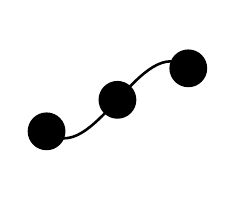
\begin{tikzpicture}[line width=1.3pt, line cap=round, line join=round, x=1mm,y=1mm]
  \draw[line width=0.93pt] (-9,-4) .. controls (-3,-9) and (3,9) .. (9,4);
  \fill (-9,-4) circle (2.4);            % the three nodes sit ON the curve,
  \fill (0,0) circle (2.4);              % at t = 0, 1/2, 1
  \fill (9,4) circle (2.4);
\end{tikzpicture}
\end{document}
